



\subsection{The L=2 case}


\begin{figure}[H]
	\centering
	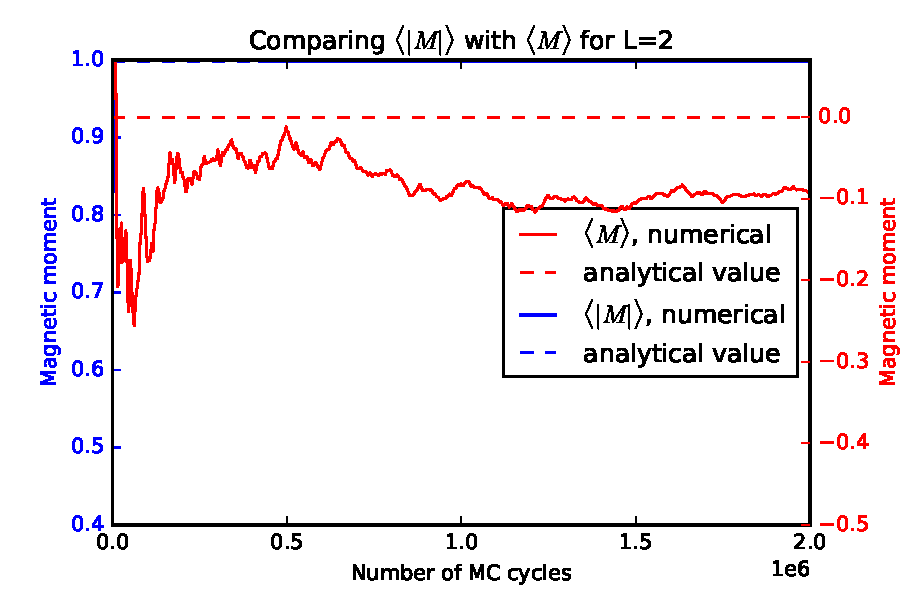
\includegraphics[width=0.7\linewidth]{../results/4b/L_2_mag_magabs}
	\caption{}
	\label{fig:l2magmagabs}
\end{figure}

Se forelesningsnotat for kommentar + diskusjon!

	
	\begin{figure}[H]
		\begin{subfigure}[b]{0.49\textwidth}
	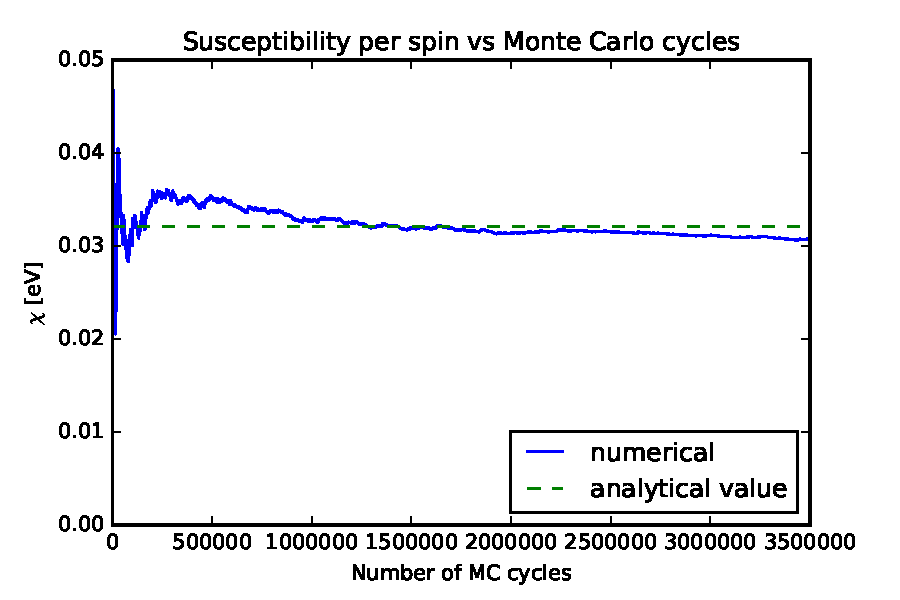
\includegraphics[width=1\linewidth]{../results/4b/L_2_susceptibility}
\caption{}
\label{fig:l2susceptibility}
		\end{subfigure}
		\hfill
		\begin{subfigure}[b]{0.49\textwidth}
		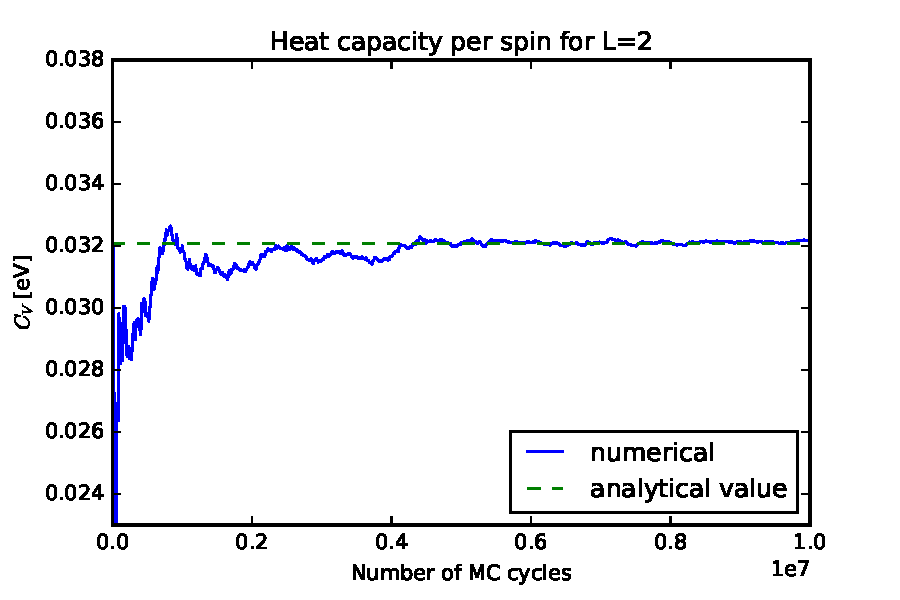
\includegraphics[width=1\linewidth]{../results/4b/L_2_heat_capasity}
\caption{}
\label{fig:l2heatcapasity}
		\end{subfigure}
		\caption{$\theta/2\theta$ scan around the (0002) peak and (0004) peak of ZnO and GaN.}
	\end{figure}

\begin{figure}[H]
	\centering
	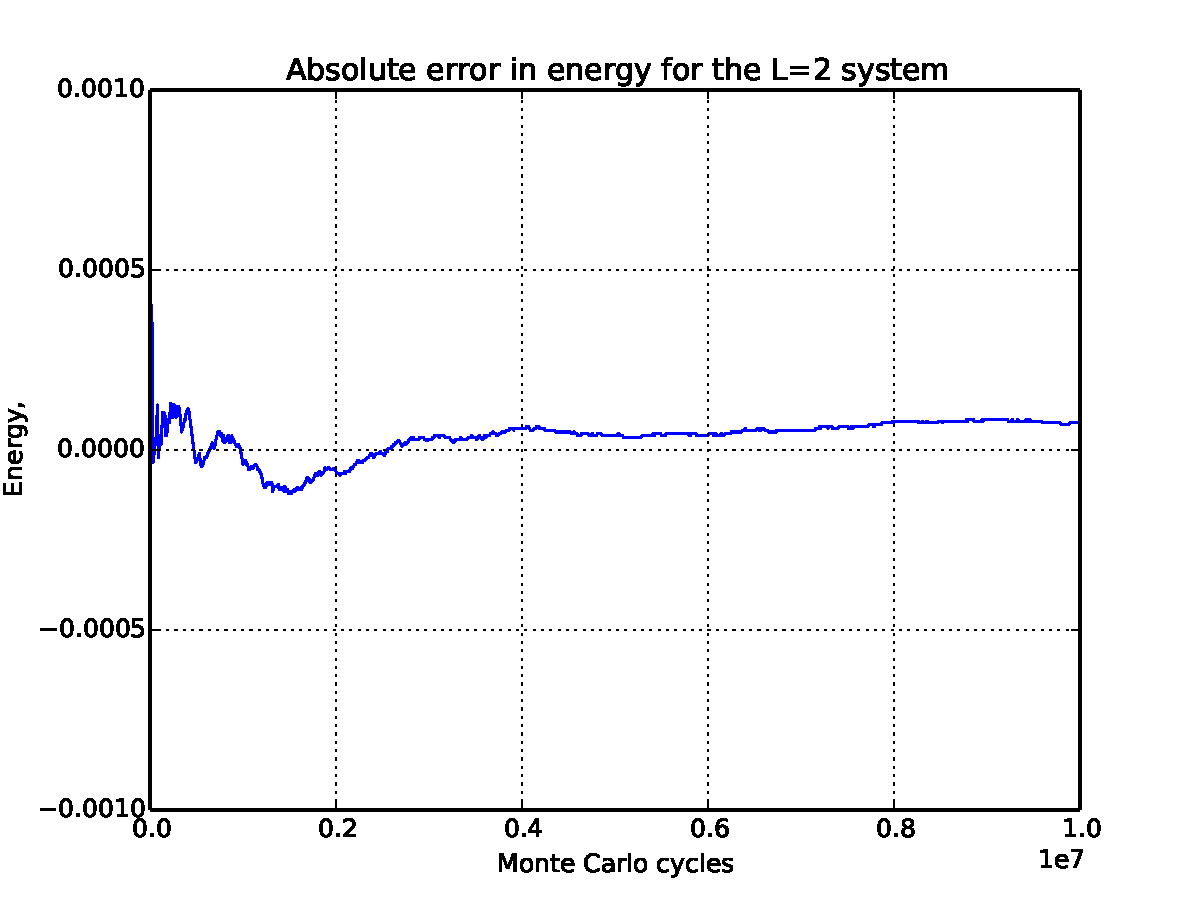
\includegraphics[width=0.7\linewidth]{../results/4b/abs_error}
	\caption{}
	\label{fig:abserror}
\end{figure}

OBS! Need an number of MC cycles necessary!

All calculations in this subsection are at T = 1.0 K. 

\begin{table}\caption{This table compares the analytical values for L=2 with the numerical ones after $10^6$ Monte Carlo cycles. The values are in units per spin.}\label{tab:compare_values}
	\begin{tabular}{ccc}
		& Numerical: & Analytical:\\ \hline
		$\left<E\right>$ &   -1.9958 & -1.9960\\
		$\left<E^2\right>$ &   15.9664 & 15.9679\\
		$\left<M\right>$ &    0.0451 & 0\\
		$\left<M^2\right>$ &    3.9930 & 3.9933\\
		$\left<|M|\right>$ &    0.9986 & 0.9987\\
		$\chi$ &   3.9849 & 3.9933\\
		$C_V$& 0.0335 & 0.0321\\
	\end{tabular}
\end{table}


\subsection{The L=20 system}

HMM: Should define an area that is enough for equilibrium!

OBS: Need the number of MC cycles to reach equilibrium!

OBS: Need equilibration time! (5 1e5?)

OBS: Comment accepted configs T dependency


\subsubsection{Initial ordering of the system}






\begin{figure}[H]
	\begin{subfigure}[b]{0.49\textwidth}
	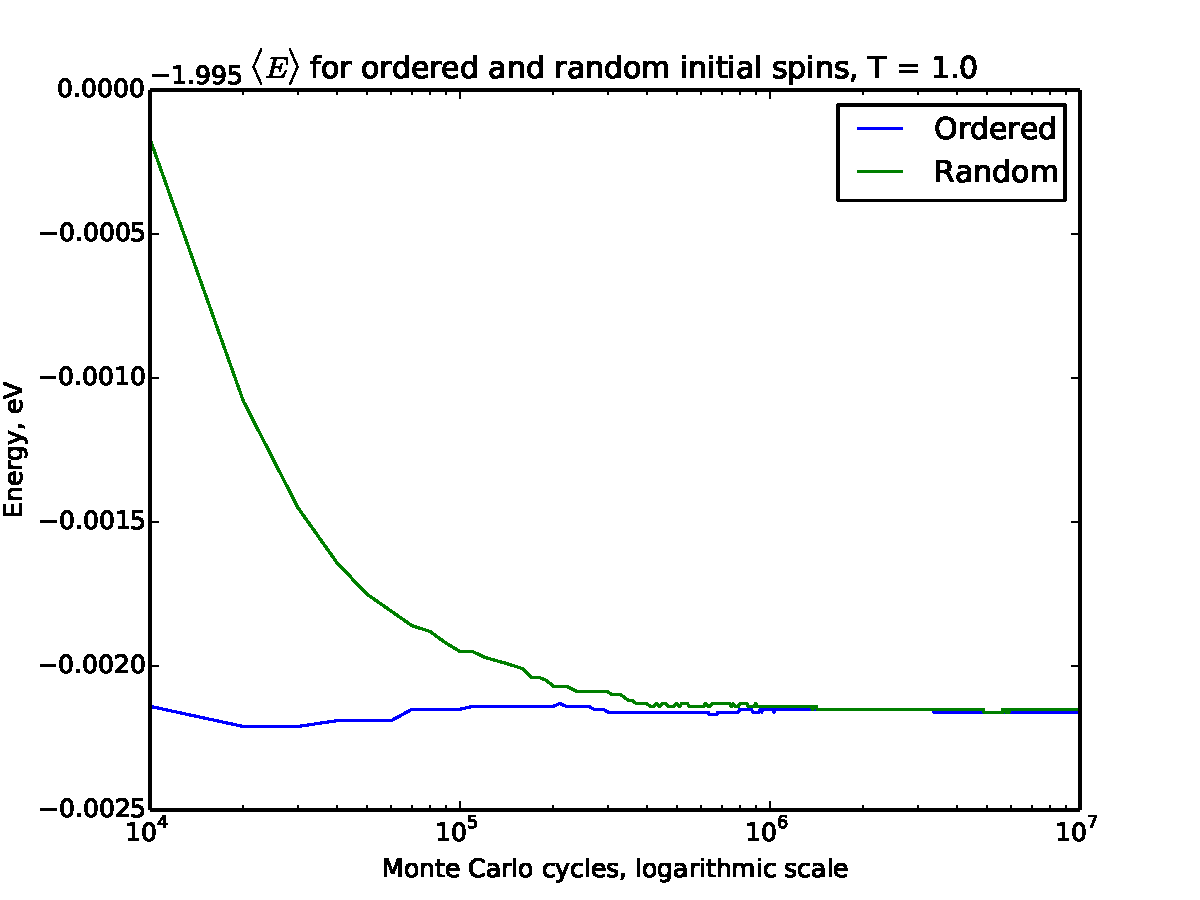
\includegraphics[width=1\linewidth]{../results/4c/ran_order_T1}
\caption{}
\label{fig:ranordert1}
	\end{subfigure}
	\hfill
	\begin{subfigure}[b]{0.49\textwidth}
	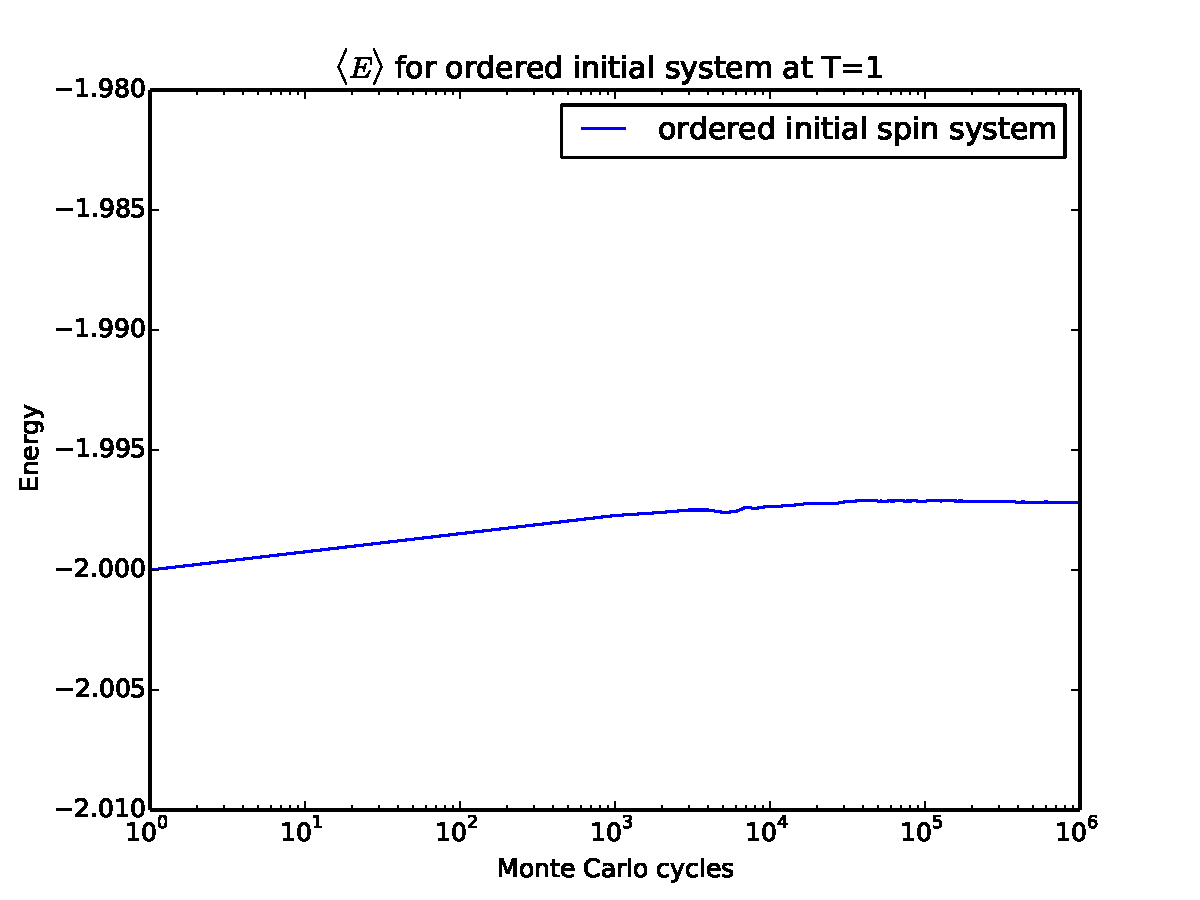
\includegraphics[width=1\linewidth]{../results/4c/order_T1_start}
\caption{}
\label{fig:ordert1start}
	\end{subfigure}
	\caption{}
\end{figure}











\begin{figure}[H]
	\centering
	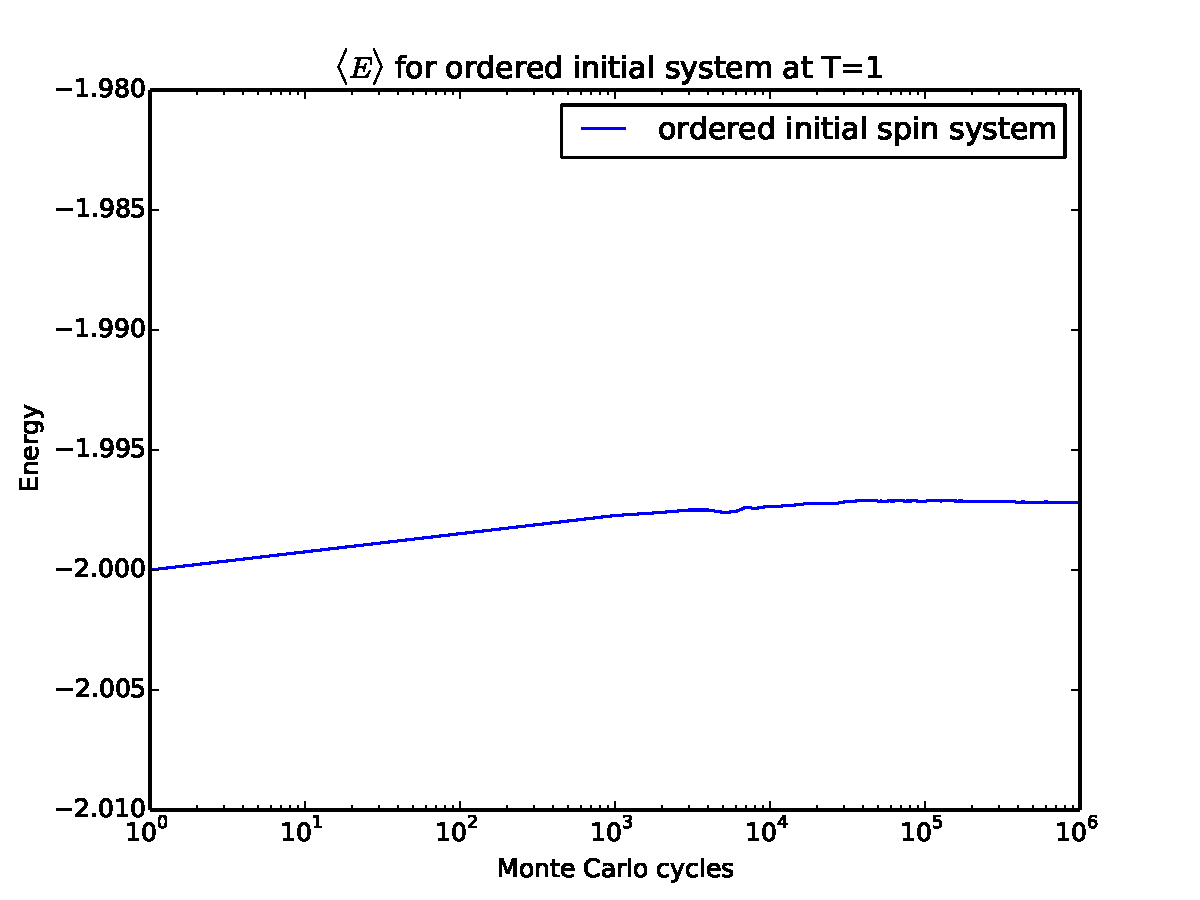
\includegraphics[width=0.7\linewidth]{../results/4c/order_T1_start}
	\caption{ Plot of the  }
	\label{fig:ranorder_t1_start}
\end{figure}
\begin{figure}[H]
		\centering
	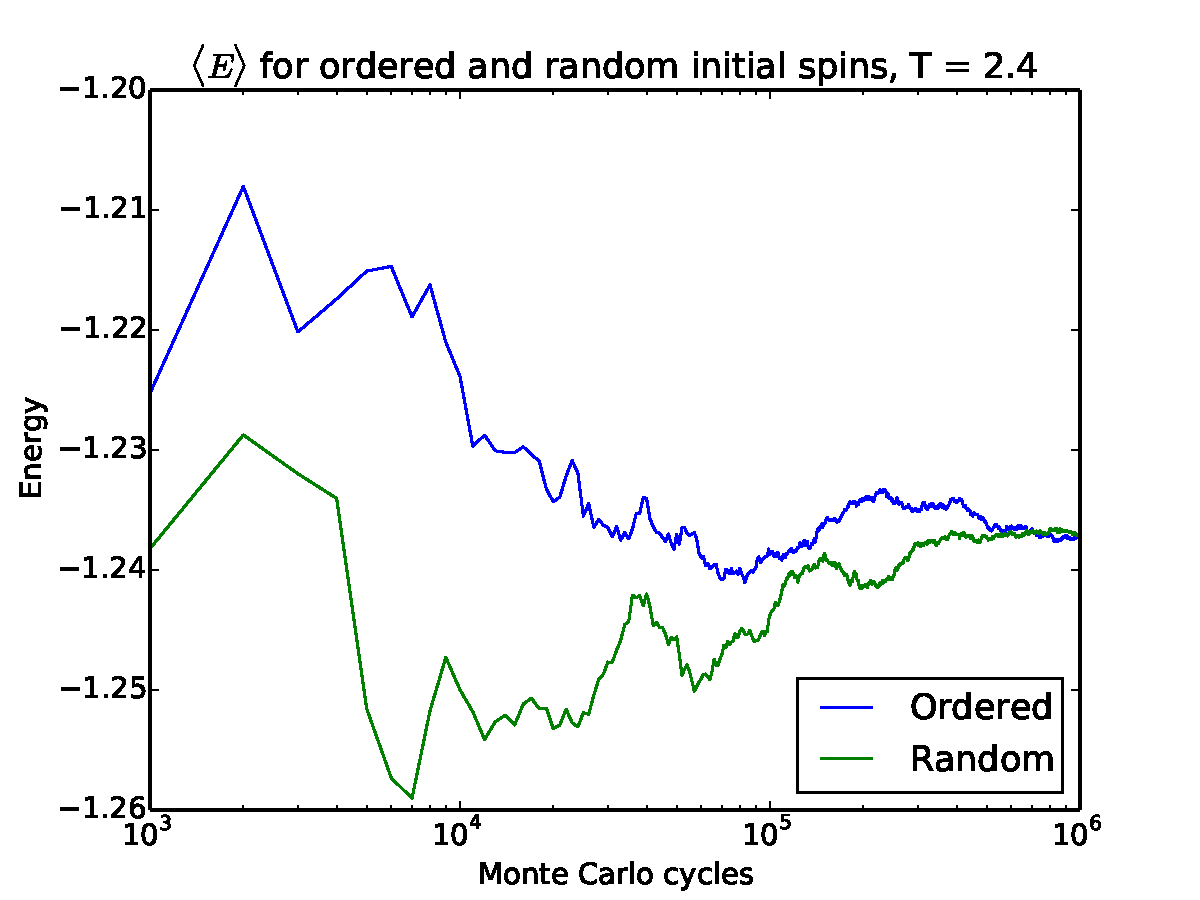
\includegraphics[width=0.7\linewidth]{../results/4c/ran_order_T2}
	\caption{}
	\label{fig:ranordert2}
\end{figure}






\subsubsection{Equilibrium time  for the random L=20 system}





	\begin{figure}[H]
	\begin{subfigure}[b]{0.49\textwidth}
		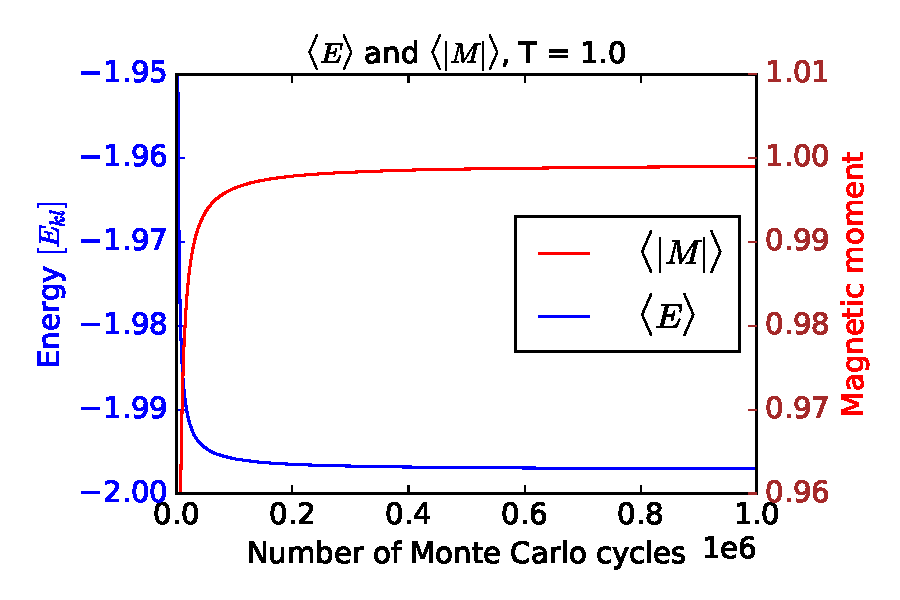
\includegraphics[width=1\linewidth]{../results/4c/En_mag_T1_0}
		\caption{}
		\label{fig:L20_mag_T_1}
	\end{subfigure}
	\hfill
	\begin{subfigure}[b]{0.49\textwidth}
		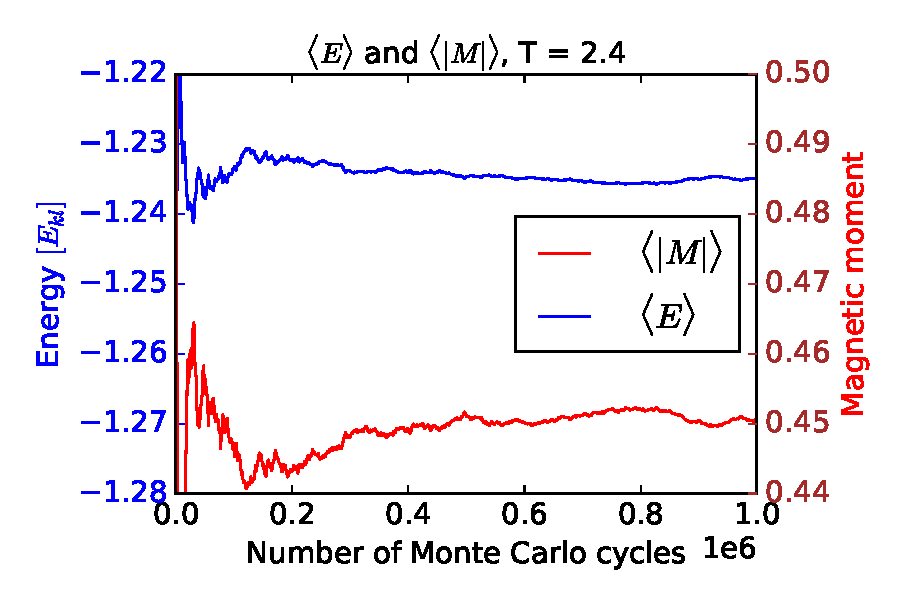
\includegraphics[width=1\linewidth]{../results/4c/En_mag_T2_4}
		\caption{}
		\label{fig:L20_mag_T_2-4}
	\end{subfigure}
	\caption{}
\end{figure}




	\begin{figure}[H]
	\begin{subfigure}[b]{0.49\textwidth}
	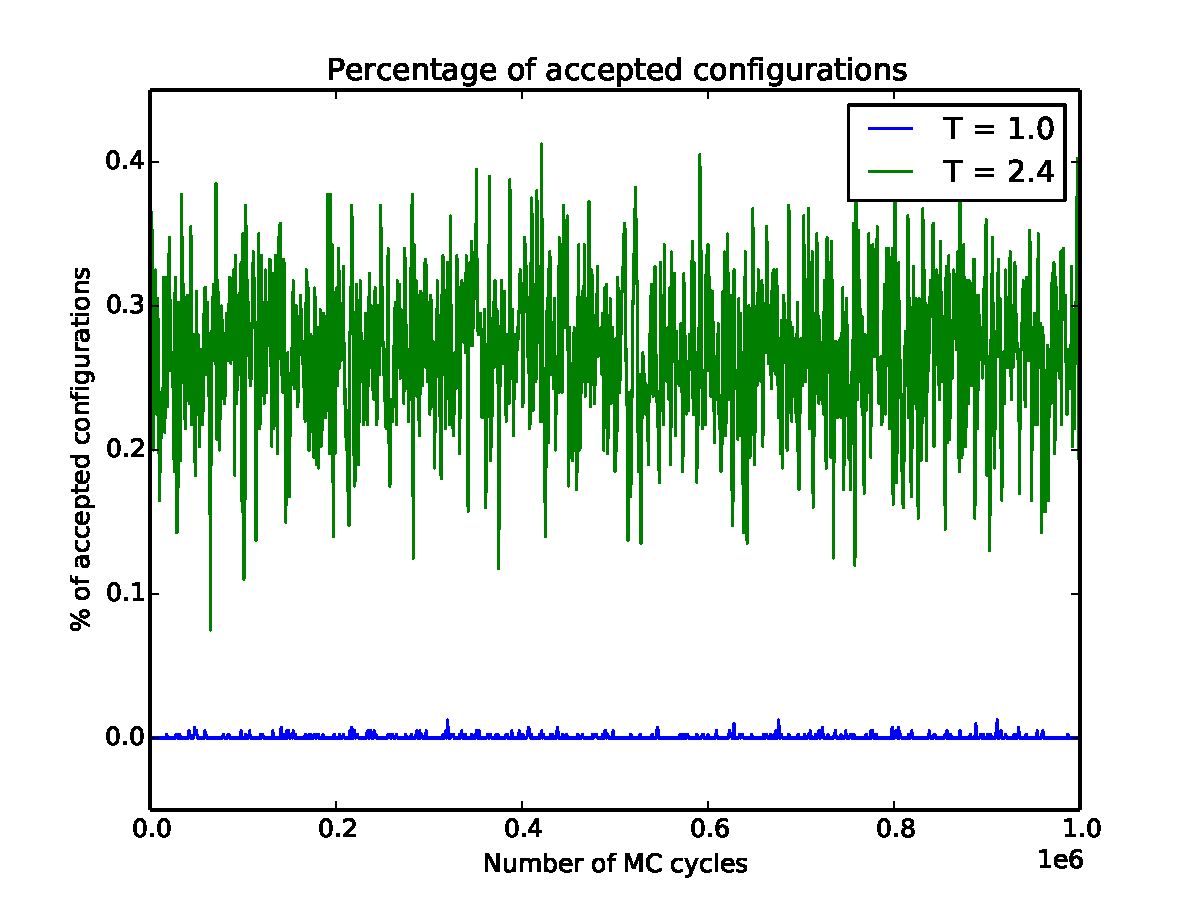
\includegraphics[width=1\linewidth]{../results/4c/L_20_accepted_configs}
\caption{}
\label{fig:l20acceptedconfigs}
	\end{subfigure}
	\hfill
	\begin{subfigure}[b]{0.49\textwidth}
	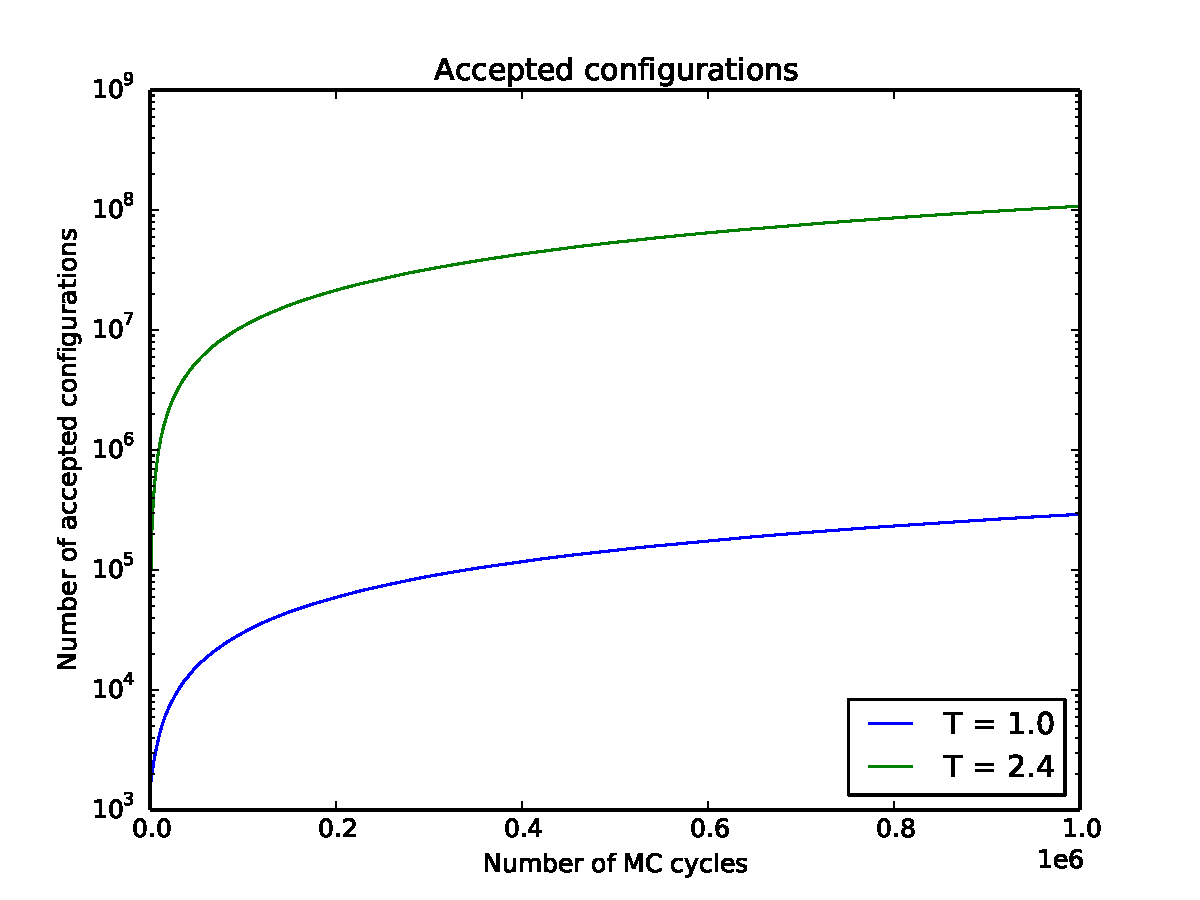
\includegraphics[width=1\linewidth]{../results/4c/L_20_accepted_configs_}
\caption{}
\label{fig:l20acceptedconfigs}
	\end{subfigure}
	\caption{}
\end{figure}











\subsubsection{Probability distrubition  for the L=20 system}


OBS: Compare result with computed variance!

OBS: Discuss behavior (In Discussion - maybe just merge result and discussion?)

Computed variance (from same dataset?):

$$ \sigma_E^2 = \left< E^2\right> - \left< E\right>^2 $$

T = 1.0 K:

$$ \sigma_E^2 = 1595.45 - (-1.997)^2 = 1591.46$$

T = 2.4 K:

$$ \sigma_E^2 =   620.734 - (-1.23759)^2
= 619.20$$



\begin{figure}[H]
	\centering
	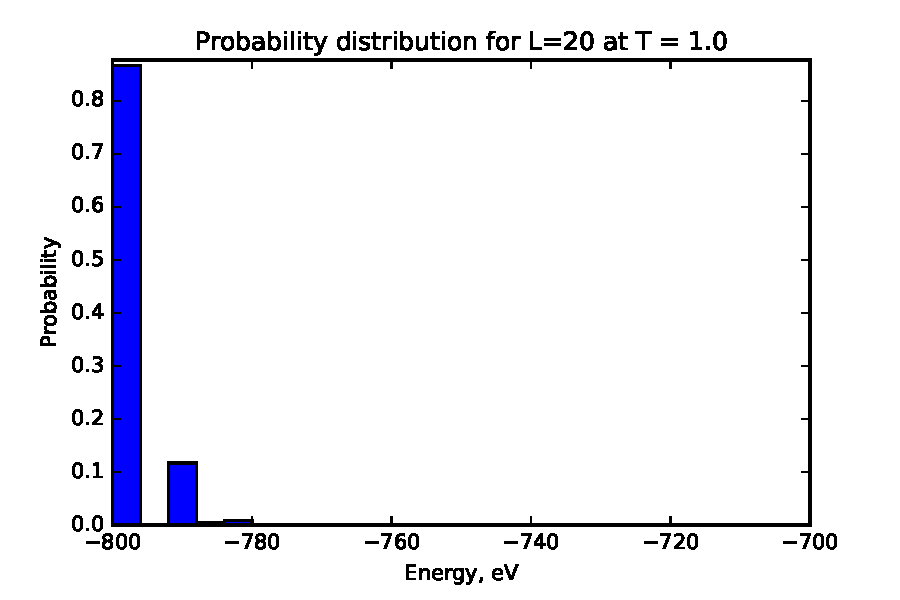
\includegraphics[width=0.7\linewidth]{../results/4d/PD_T_1MC_1e6}
	\caption{}
	\label{fig:pdt1}
\end{figure}

\begin{figure}[H]
	\centering
	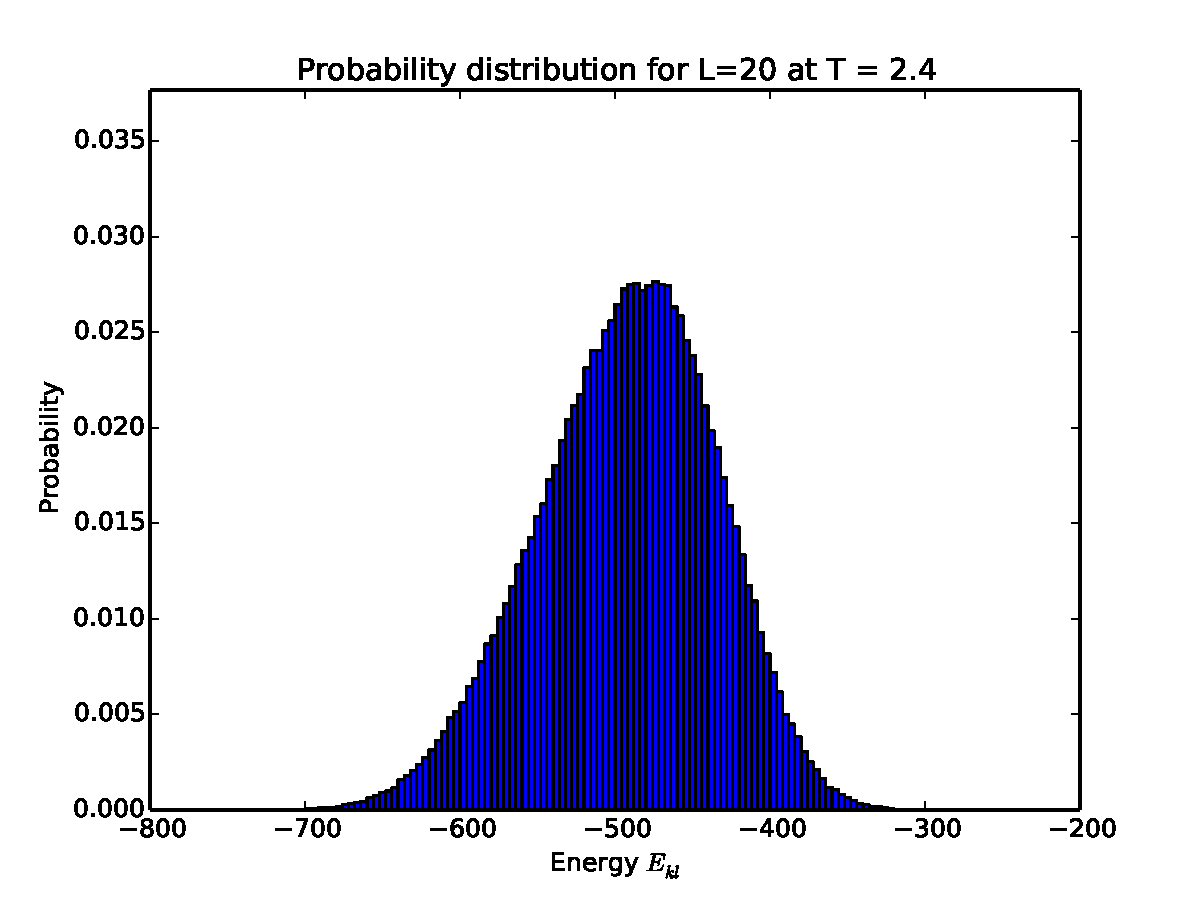
\includegraphics[width=0.7\linewidth]{../results/4d/PD_T_2MC_1e6}
	\caption{}
	\label{fig:pdt2_4}
\end{figure}



\subsection{Phase transition and Critical temperature}



OBS: Plot of E, M, Cv, X as functions of T (put L as legend and plot together)

OBS: Indication of phase transition? (Peak - at least for Cv and X)

OBS: Use Equation \ref{eq:critical_T} to extract $T_C$.


Timing parallellisering

	\begin{figure}[H]
	\begin{subfigure}[b]{0.5\textwidth}
	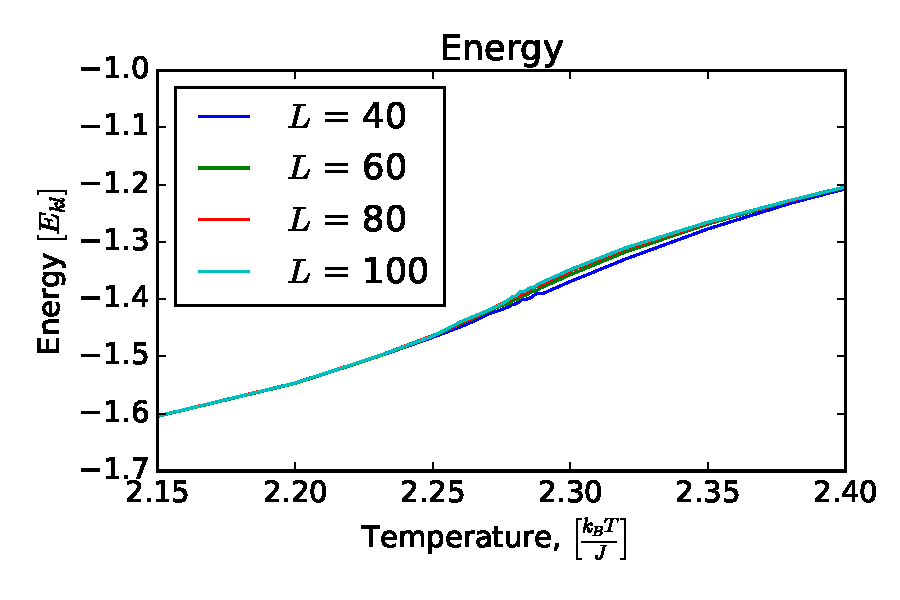
\includegraphics[width=1\linewidth]{../results/4e/4e_energy}
\caption{}
\label{fig:4eenergy}
	\end{subfigure}
	\hfill
	\begin{subfigure}[b]{0.5\textwidth}
	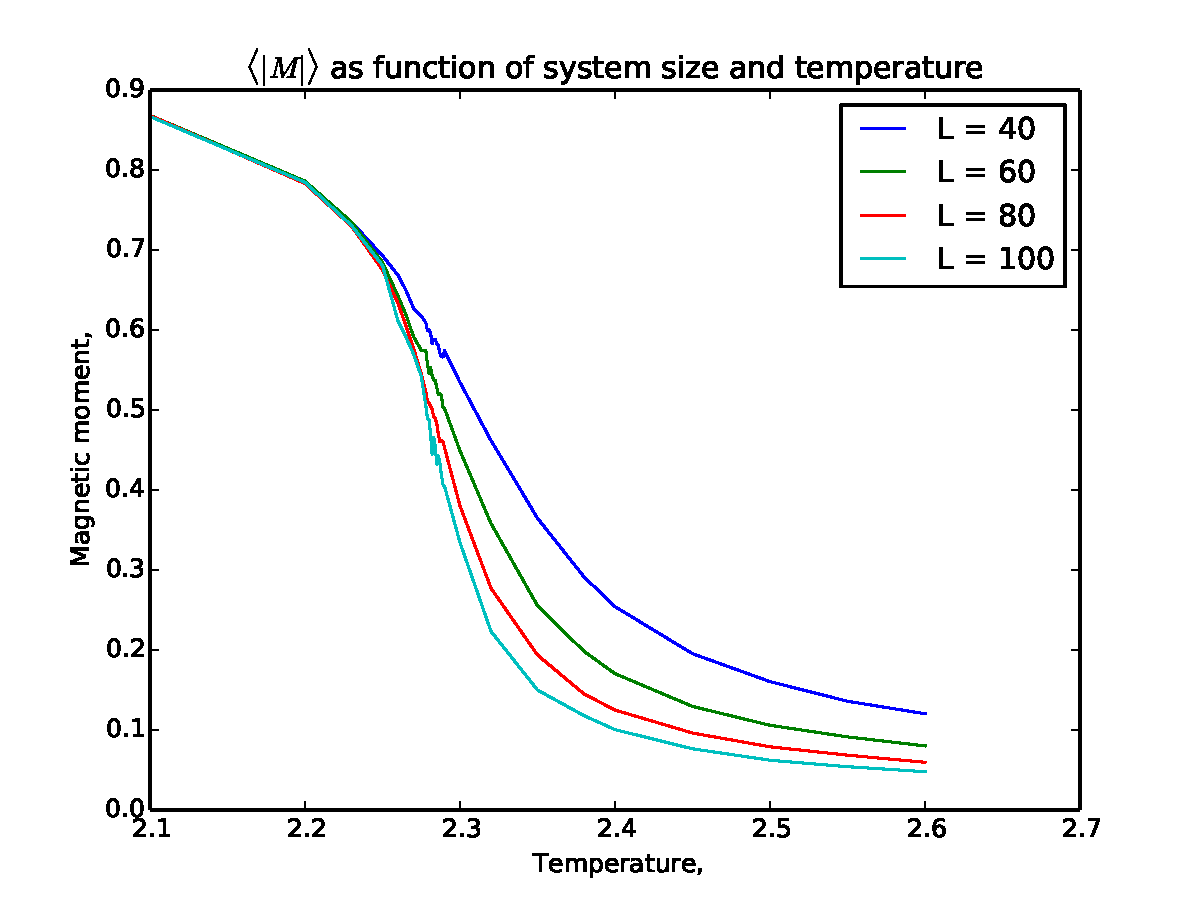
\includegraphics[width=1\linewidth]{../results/4e/4e_mag}
\caption{}
\label{fig:4emag}
	\end{subfigure}
	\caption{}
\end{figure}




\begin{figure}[H]
	\centering
	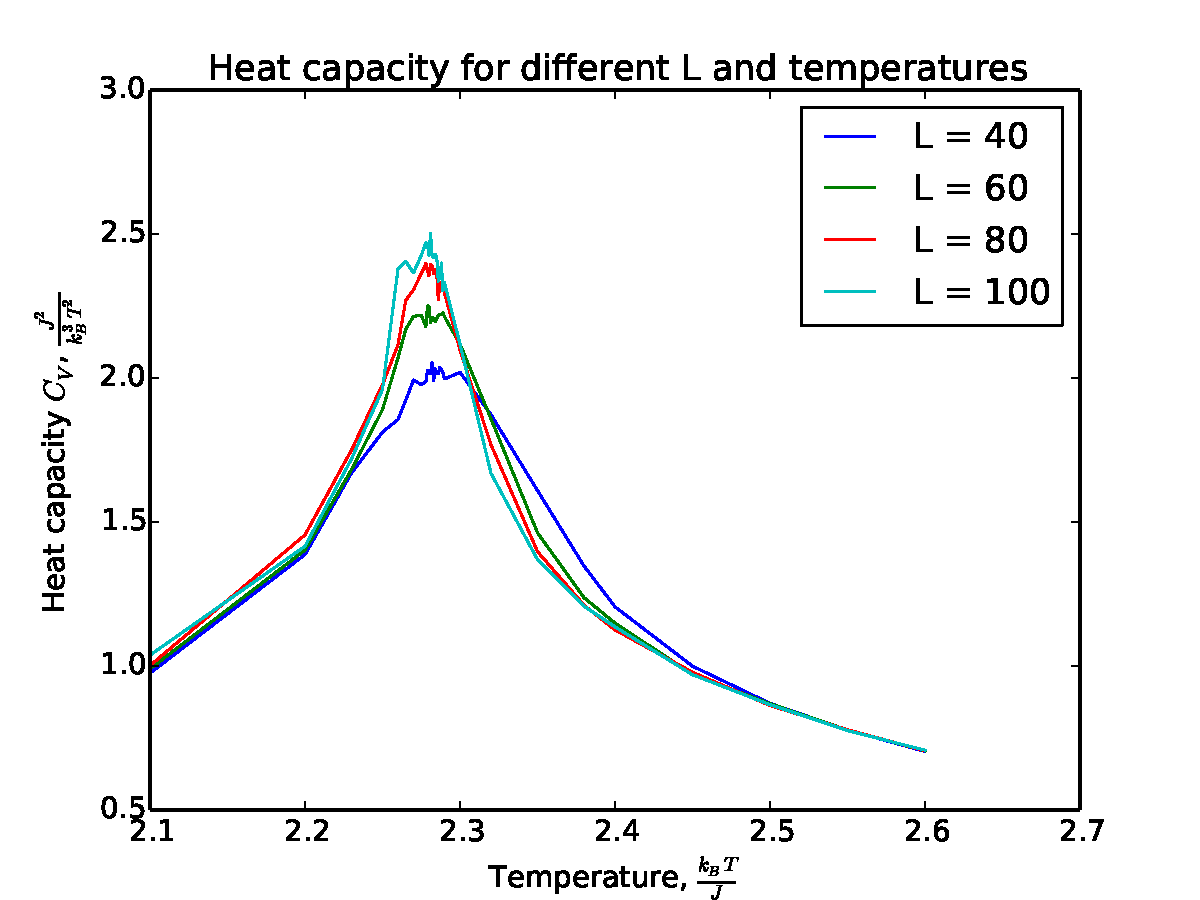
\includegraphics[width=0.7\linewidth]{../results/4e/4e_Cv}
	\caption{}
	\label{fig:4ecv}
\end{figure}

\begin{figure}[H]
	\centering
	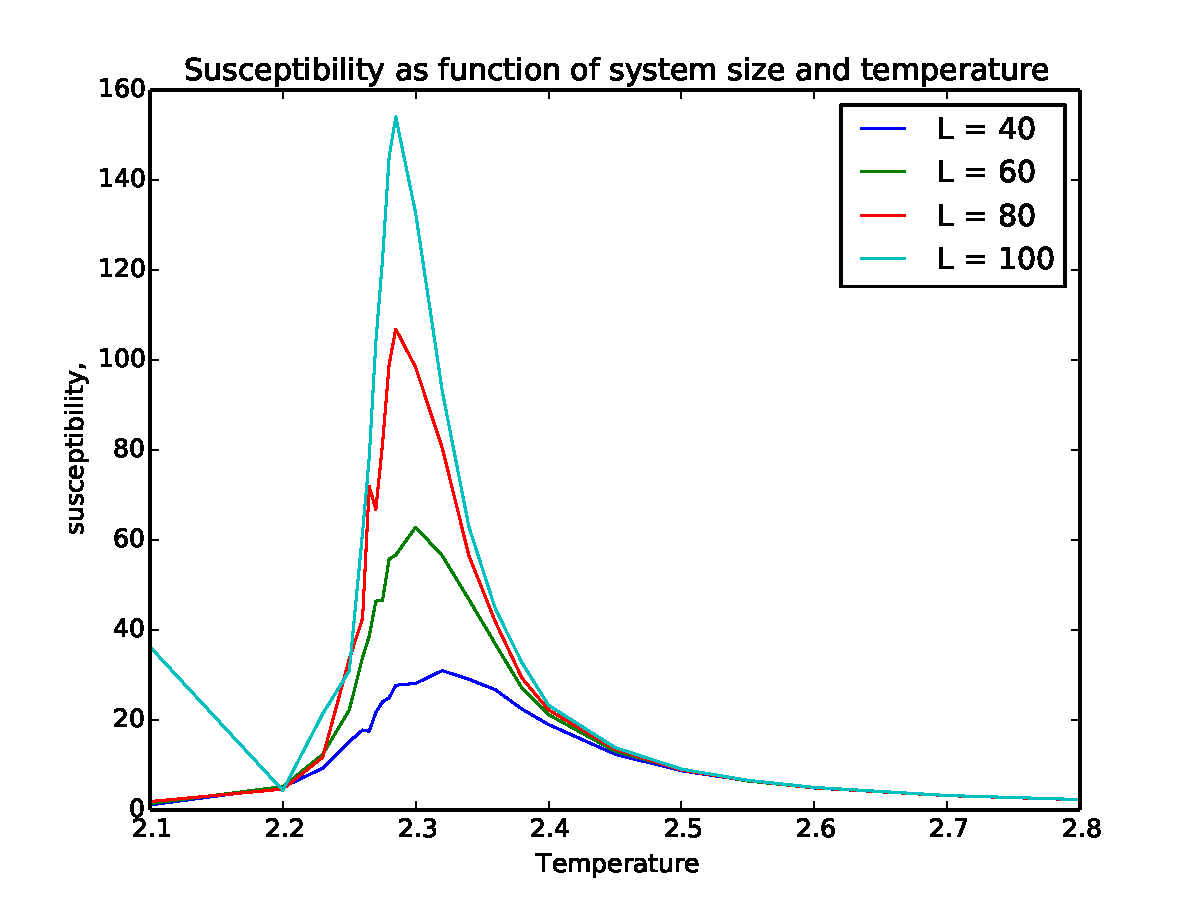
\includegraphics[width=0.7\linewidth]{../results/4e/4e_x}
	\caption{}
	\label{fig:4ex}
\end{figure}


\begin{table}[H]
	\caption{text}
	\label{tab: T_C}
	\begin{tabular}{cccccc}
		 L & $T_C$ \\ \hline    
     40 & 2.282 \\ 
 60 & 2.279 \\ 
 80 & 2.278 \\ 
 100 & 2.281 \\ 

	\end{tabular}
\end{table}




Exact $T_C =  kTC/J = 2/ \ln(1+\sqrt{
	2}) \approx 2.269$ \cite{Onsager}

\begin{table}\caption{L=80 and MC cycles is 1e6.}
	\begin{tabular}{cc}
		Number of processors:& CPU time [s]: \\ \hline
		1 & 513.069\\
		2 & 306.975\\
	\end{tabular}
\end{table}
